\chapter[A TADR PROTEIN MUTATION]{MUTATION OF A TADR PROTEIN LEADS TO RHODOPSIN AND G$_{\texttt{q}}$-DEPENDENT RETINAL DEGENERATION IN \textit{DROSOPHILA}}                     % MUST be CAPITALIZED

The work presented in this chapter is reproduced from a study by Ni et al., published in J. Neurosci. \cite{Ni2008}

This work was conducted under the direction of Dr. Hong--Sheng Li and it is with gratitude to him and the other authors that I reproduce these data for the purpose of this dissertation. My contribution in this work was to execute the majority of the experiments including mapping the mutation, generating transgenic fly and double mutants, optical neutrolization analysis, toluidine blue staining, immunostaining, electroretinaogram recordings, glutathione--Sepharose binding assay, Arr2 binding and releasing assays, light--stimulated GST$\gamma$S binding assay and light--dependent G$_{\texttt{q}}$ localization assay.  Peiyi Guo contributed by conducting the whole--cell recordings. Keith Reddig contributed by conducting electron microscopy and sectioning samples for toluidine blue staining. Mirna Mitra contributed by mapping the mutation. Dr. Hong--Sheng Li did the EMS screen. Dr. Hong--Sheng Li and I prepared the manuscript together.
\clearpage

%%% Abstract %%%

\section{Abstract}
The \textit{Drosophila} photoreceptor is a model system for genetic study of retinal degeneration.  Many gene mutations cause fly photoreceptor degeneration, either due to excessive stimulation of the visual transduction (phototransduction) cascade, or through apoptotic pathways that in many cases involve a visual arrestin Arr2.  Here we report a gene named \textit{tadr} (for \underline{t}orn \underline{a}nd \underline{d}iminished \underline{r}habdomeres), which, when mutated, leads to photoreceptor degeneration through a different mechanism. Degeneration in the \textit{tadr} mutant is characterized by shrunk and disrupted rhabdomeres, the light sensory organelles of photoreceptor. The TADR protein interacted in vitro with the major light receptor Rh1 rhodopsin, and genetic reduction of the Rh1 level suppressed the \textit{tadr} mutation--caused degeneration, suggesting the degeneration is Rh1--dependent.  Nonetheless, removal of phospholipase C (PLC), a key enzyme in phototransdction, and that of Arr2 failed to inhibit rhabdomeral degeneration in the \textit{tadr} mutant background.  Biochemical analyses revealed that, in the \textit{tadr} mutant, the G$_{\texttt{q}}$ protein of Rh1 is defective in dissociation from the membrane during light stimulation.  Importantly, reduction of G$_{\texttt{q}}$ level by introducing a hypomorphic allele of G$\alpha$q gene greatly inhibited the \textit{tadr} degeneration phenotype.  These results may suggest that loss of a potential TADR--Rh1 interaction leads to an abnormality in the G$_{\texttt{q}}$ signaling, which in turn triggers rhabdomeral degeneration independent of the PLC phototransduction cascade.  We propose that TADR--like proteins may also protect photoreceptors from degeneration in mammals including humans.
\textbf{keywords:} Retinal degeneration, Rhodopsin, G protein, Photoreceptor, \textit{Drosophila}, GPCR, Cation amino acid transporter

\section{Introduction}
Degeneration of rod and/or cone photoreceptors is a defining characteristic of retinitis pigmentosa (RP), a subset of human hereditary retinal diseases \cite{Yamamoto1997} that cause night blindness followed by progressive loss of vision \cite{Hartong2006}.  Many identified causal genes of RP encode key components of the visual transduction (phototransduction) cascade in photoreceptors \cite{Hartong2006,Daiger2007}.  For instance, mutation in the light receptor rhodopsin is a prevalent cause of autosomal dominant RP \cite{Kaushal1994,Dryja2000,Wilson2003}, and loss of rhodopsin regulatory proteins, arrestins and a rhodopsin kinase, causes Oguchi disease, an autosomal recessive form of RP \cite{Fuchs1995,Yamamoto1997,Dryja2000}.  In addition, several other RP genes are required for the trafficking and maturation of rhodopsin molecules \cite{Hartong2006}.  Thus, abnormalities in rhodopsin signaling pathways are major causes of photoreceptor degeneration.  Nonetheless, in many RP cases, it remains puzzling why the product of an affected gene is important for photoreceptor protection.  More importantly, the mutant genes in about 40\% of RP cases have yet to be identified \cite{Hartong2006,Daiger2007}.

The \textit{Drosophila} photoreceptor is a genetic model system for the study of both phototransduction \cite{Montell1999,Hardie2001} and retinal degeneration \cite{Ranganathan2003}. The whole visual transduction cascade is localized in a packed microvillar structure rhabdomere \cite{Hardie2001}, which is analogous to the outer segment of rod and cone photoreceptors.  The fly rhodopsin is coupled to a G$_{\texttt{q}}$ type G protein \cite{Lee1994,Scott1995}.  Instead of activating phosphodiesterase (PDE) to close cGMP--gated channels as in mammalian photoreceptors, this fly visual G protein stimulates a \textit{norpA} gene--encoded phospholipase C (PLC) to open TRP Ca$^{2+}$/cation channels \cite{Bloomquist1988,Hardie1992,Montell1999}.  To rapidly terminate the light response, the stimulated rhodopsin molecule is deactivated promptly through a visual arrestin Arr2 \cite{Dolph1993} and a dCAMTA/dFbxl4 pathway \cite{Han2006}.
  
Similar to those in humans, fly mutations in phototransduction molecules including rhodopsin \cite{Leonard1992,Kurada1995,Iakhine2004}, PLC \cite{Meyertholen1987,Zinkl1990,Alloway2000}, TRP \cite{Hong2002,Wang2005} and arrestins \cite{Dolph1993,Satoh2005} all cause age--dependent photoreceptor degenerations, which are generally characterized by diminished rhabdomeres.  Several other visual proteins such as a diacylgrycerol kinase RDGA and a rhodopsin phosphatase RDGC are also essential for photoreceptor protection \cite{Masai1993,Kiselev2000}. Fly photoreceptors may degenerate in a necrotic, Ca$^{2+}$--dependent manner due to prolonged stimulation of the phototransduction cascade, or through apoptotic processes \cite{Wang2007}.  In several mutants including \textit{rdgC} and \textit{norpA}, rhodopsin forms a stable complex with Arr2 to trigger photoreceptor apoptosis \cite{Alloway2000,Kiselev2000}.  Here we report the isolation of a mutant fly \textit{tadr} that undergoes rhabdomeral degeneration through a new pathway. 

\section{Materials and Methods}
\subsection{Fly genetics}
The genotype of wild--type flies is cn,bw unless mentioned otherwise in the text.  The \textit{tadr} mutant was generated from cn progenitors using the chemical mutagen ethyl methanesulfonate (EMS), and recombined into a cn,bw background.  Except for the dark--reared flies that were never exposed to light from the prepupal stage, all others were raised in an approximate 12 hr light ($\sim$250 lux) /12 hr dark cycle.  The mutant alleles of other genes used in this work are \textit{ninaE}$^5$, \textit{arr2}$^5$, \textit{norpA}$^{24}$, G$_{\alpha\texttt{q}}^{1}$, and \textit{glass}$^2$.

A wild--type \textit{CG9264} cDNA was obtained through RT--PCR, subcloned into a pCaSpeR--\textit{hs} vector, and injected into w$^{1118}$ flies to generate \textit{p[hs--CG9264]} transgenic flies.  The transgene was subsequently crossed into the \textit{tadr} mutant background.  To express the protein, flies were heat shocked for 1 hr at 37$^{\circ}\mathrm{C}$ in a water bath once a day from late pupal stage and examined at 7--days old.

\subsection{Optical neutralization analysis}
This analysis was performed as described previously \cite{Franceschini1971}.  In brief, fly heads were separated from the body and immersed in a layer of lens oil to optically neutralize the cornea.  On the stage of a microscope, a spotlight was shone into the head from the neck side for antidromic illumination of the compound eye.  The rhabdomeres that appeared as bright dots due to high transmission of light were counted for each upright ommatidium.  The mean number of rhadomeres per ommatidium was calculated for each genotype and condition based on the results of 30 ommatidia from 5 flies.  Standard errors of means (SEMs) were presented as error bars in figures.

\newpage
\begin{figure}
	\centering
		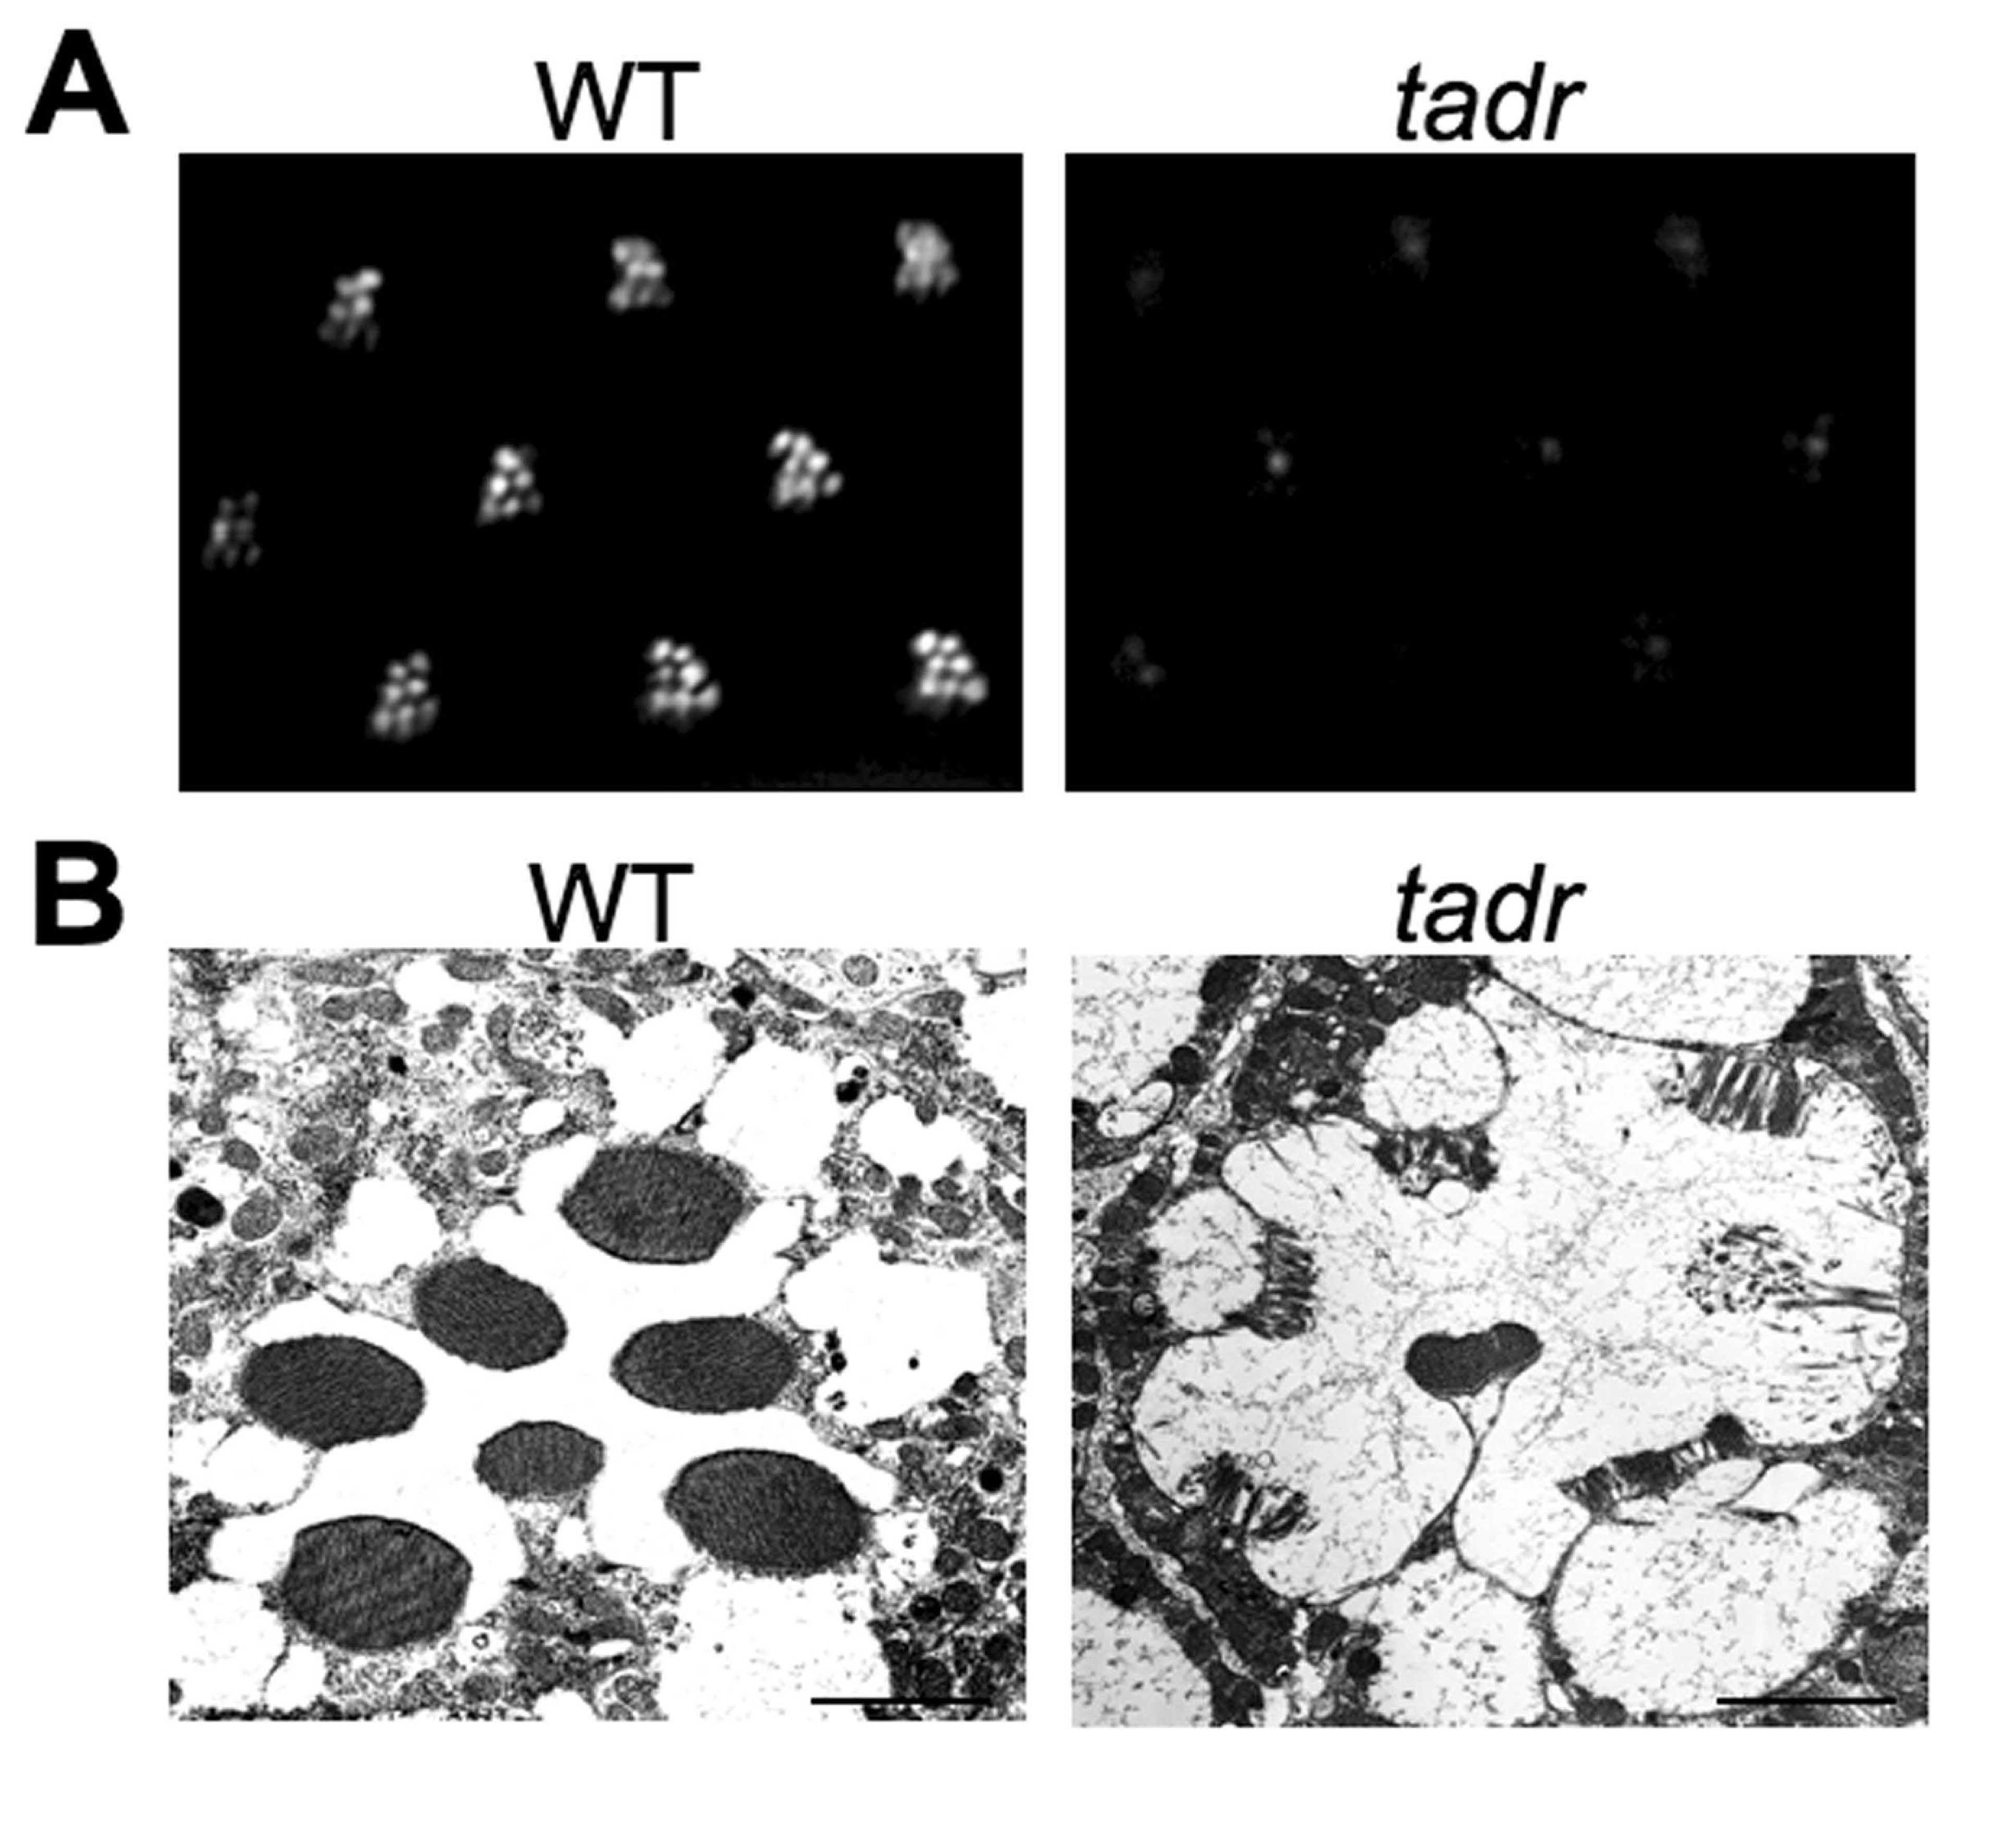
\includegraphics[width=\textwidth]{fig2-1.eps}
	\caption[Short caption for the List of Figures]{leave here blank}
	\label{fig2-1}
\end{figure}
\clearpage \Fref{fig2-1}--- A longer caption which is more descriptive would go here.\clearpage

\begin{table}
\caption[Short caption for the List of Table]{leave here blank}
	\centering
		\begin{tabular}{ll}
			\hline\\
			\textbf{Primer Name}	& \textbf{Primer sequence (5'$\rightarrow$3')}\\ 
			\hline\\
			T4-f	& GGAATTCcatatgGCCTCCTCCG\\
			T4-r	& CGgctagcTTGGATTCTCACC\\
			Pl-T4-f	& GCGcctaggCGGTGTTGACATAAATAC\\
			Pl-T4-r	& GCGcctaggacgtcTAGCTTGGATTCT\\
			PlPr-T4-f	& GCGcctaggTAACACCGTGCGTG\\
			pSC101*-f	& GCATGCaagcttGGCGTAATCATGGTCATAG\\
			pSC101* -r	& TGATAATTactagtCCTTTTcccgggagatctGGGTATCTG\\
			par-pSC101*-f & TCCCCGCGGACAGTAAGA\\
			par-pSC101*-r & CCTATTAATCATCTGTGCATATGGACA\\
			\hline\\
		\end{tabular}
	\label{tab:Oligo}
\end{table}
\clearpage \Tref{tab:Oligo}--- A longer caption which is more descriptive would go here.\clearpage